\chapter{固体中的电子}\label{ch:b3:electrons-in-solids}

% Provenance (not for print): second half of the "physique du solide"
% module (Drude, Sommerfeld, bands, semiconductors) common to the
% surveyed third-year curricula.

铜的导电能力比石英高出一亿亿亿倍，
这是所有物理性质中跨度最大的——而造成此差距的，
竟是两种外观上都像灰色石块的材料。上一章的骨架
对此毫无解释；注入其中的\emph{电子}
却解释了全部。本章依次考察本世纪对这一问题的三次尝试，
每一次都继承了前一次留下的烂摊子：德鲁德的经典
弹子球模型（1900 年），它正确给出欧姆定律，却把热容
算错得离谱；索末菲的费米气体，是
\cref{ch:b3:quantum-statistics}为它兑现“支票”；而布洛赫的
洞见是：周期晶格中的电子波会像其他任何波一样发生布拉格反射，
从而打开\emph{带隙}，将所有固体分成
\omterm{def:b3:electrons-in-solids:classes}{金属}、\omterm{def:b3:electrons-in-solids:classes}{绝缘体}，以及窄带隙的“中间孩子”，
即\omterm{def:b3:electrons-in-solids:classes}{半导体}，整个电子时代都建立在它之上。本章
以一块太阳能电池板的内部收尾。

\section{德鲁德的弹子球金属}

\begin{proposition}[德鲁德电导率]\label{prop:b3:electrons-in-solids:drude}
\index{德鲁德模型}\index{电导率!微观}\index{漂移速度}
将\omterm{def:b3:electrons-in-solids:classes}{金属}的价电子视为经典气体，数密度为 $n$，
每隔 $\tau$ 秒与障碍物碰撞一次。电场 $\vect E$
在两次碰撞之间使每个电子加速，其平均\emph{\omterm{prop:b3:electrons-in-solids:drude}{漂移
速度}}为 $\vect v_{\text{d}} = -e\tau\vect E/m_{\text{e}}$，
与热运动相比微不足道。电流密度 $\vect j =
-ne\vect v_{\text{d}}$ 于是局域地服从欧姆定律，
$\vect j = \sigma\vect E$，其中
\[
\sigma = \frac{ne^2\tau}{m_{\text{e}}} .
\]
铜的实测 $\sigma$ 要求 $\tau \approx \qty{2.5e-14}{s}$
——该模型的两大成就由此而来：其一，它解释了电阻器
为何发热（电场做功在每次碰撞中都转化为热），其二，它
预言了维德曼–弗兰兹定律，即 $\kappa/\sigma T$ 在所有\omterm{def:b3:electrons-in-solids:classes}{金属}中
都是同一常数——电子既携带电荷，也输运热量
（见\cref{exo:b3:electrons-in-solids:5}）。
\end{proposition}

\begin{proof}
两次碰撞之间有 $\dot{\vect v} = -e\vect E/m_{\text{e}}$；
每次碰撞后从零开始重新计算，在一段
平均时间 $\tau$ 内获得的平均速度为 $-e\tau\vect E/m_{\text{e}}$。于是 $\vect j =
-ne\vect v_{\text{d}} = (ne^2\tau/m_{\text{e}})\vect E$。
\end{proof}

\begin{omfigure}
\begin{tikzpicture}[scale=1.0]
  % ion grid
  \foreach \x in {0,1.3,...,7.9}
    \foreach \y in {0,1.1,2.2}
      \draw[omDef!50, fill=omDef!12] (\x,\y) circle (5.5pt);
  % zigzag electron path with slight downfield drift
  \draw[omThm, thick, ->]
    (0.25,1.62) -- (1.0,0.55) -- (1.9,1.7) -- (2.6,0.6) -- (3.6,1.55)
    -- (4.3,0.45) -- (5.25,1.6) -- (5.95,0.5) -- (6.9,1.5) -- (7.65,0.7);
  % field and drift arrows
  \draw[->, thick] (2.6,3.0) -- (1.2,3.0)
    node[midway, above, font=\scriptsize] {$\vect E$};
  \draw[->, thick, omThm, dashed] (5.0,3.0) -- (6.8,3.0)
    node[midway, above, font=\scriptsize]
    {漂移 $\vect v_{\text{d}}$};
\end{tikzpicture}

{\small 德鲁德的图景：电子以
$\sim\qty{e6}{m/s}$ 的速度来回碰撞，而电场只叠加上
零点几毫米每秒的漂移
（见\cref{exo:b3:electrons-in-solids:2}）。欧姆定律由此自然得出；该模型的
失败还带来了更多启示。}
\end{omfigure}

\begin{remark}[索末菲的补救]\label{rem:b3:electrons-in-solids:sommerfeld}
\index{索末菲模型}\index{费米能!金属中}
德鲁德气体本应使每个电子给\omterm{def:b3:electrons-in-solids:classes}{金属}热容带来 $\tfrac32k_{\text{B}}$ 的贡献，
而实验测得的贡献却小了一百倍。
\Cref{ch:b3:quantum-statistics}早已为电子洗脱了罪名：
它们是\emph{简并费米气体}，$T_{\text{F}} \sim
\qty{8e4}{K}$，只有距费米面
$k_{\text{B}}T$ 以内的电子才能响应——对热，
也对散射。索末菲以费米–狄拉克统计重做德鲁德
统计，保留了电导率公式（其中 $\tau$ 现在是
费米面电子的寿命，其速率 \qty{e6}{m/s} 即
$v_{\text{F}}$，而非热运动速率），并将热容修正为其
实测的 $T/T_{\text{F}}$ 那一小部分，甚至修补了
维德曼–弗兰兹的数值常数。每一个自由电子模型仍留下一个谜
：为何石英竟完全不导电。
\end{remark}

\section{布洛赫：晶格开口说话}

\begin{theorem}[布洛赫态与带隙]\label{thm:b3:electrons-in-solids:bloch}
\index{布洛赫定理}\index{带隙}\index{能带结构}
在完美的周期势中，定态为
\emph{布洛赫波} $\psi_k(x) = u_k(x)\eu^{\iu kx}$——
即以晶格自身周期性 $u_k$ 修饰的平面波——
它们可以\emph{无散射地}传播：完美\omterm{def:b3:crystalline-solids:lattice}{晶体}的
电阻为零，而实际电阻来自缺陷
（振动、杂质）。但并非所有能量都允许存在。在
$k = \pi/a$ 处电子的波长为 $2a$：晶格上的布拉格条件
（见\cref{thm:b3:crystalline-solids:dispersion}，
对声波也曾有过同样的发现）。反射波与入射波
形成两种驻波图样——电荷堆积在离子上
（能量较低）或位于离子之间（能量较高）——于是自由电子
抛物线 $E = \hbar^2k^2/2m_{\text{e}}$ 被撕开：出现一段
禁戒能量区间，即\emph{带隙} $E_{\text{g}}$，将
已填满允许态的\emph{能带}与下一条分开。一个
\omterm{def:b3:crystalline-solids:lattice}{晶体}的电子身份，便是其能带与带隙构成的阶梯。
\end{theorem}
\admitted

\begin{omfigure}
\begin{tikzpicture}
  \begin{axis}[omaxis, axis x line=bottom, axis y line=left,
    width=9.6cm, height=6.2cm, xmin=0, xmax=5.4, ymin=0, ymax=2.6,
    xlabel={$k$}, ylabel={$E$},
    xlabel style={at={(axis description cs:0.5,-0.1)}, anchor=north},
    xtick={3.1416}, xticklabels={$\pi/a$}, ytick=\empty, clip=true]
    % free-electron parabola (dashed)
    \addplot[gray, dashed, domain=0:5.1, samples=120] {x*x/10};
    % lower band: bends flat at zone edge
    \addplot[omDef, very thick, domain=0:3.1416, samples=120]
      {x*x/10 - 0.18*(x/3.1416)^6};
    % upper band
    \addplot[omDef, very thick, domain=3.1416:5.1, samples=120]
      {x*x/10 + 0.18*((5.1-x)/1.9584)^2};
    \draw[gray, dashed] (axis cs:3.1416,0) -- (axis cs:3.1416,2.55);
    % gap markers
    \draw[omThm, thick, <->] (axis cs:3.2,0.81) -- (axis cs:3.2,1.16);
    \node[omThm, font=\scriptsize, anchor=west] at (axis cs:3.34,0.98)
      {带隙 $E_{\text{g}}$};
    \node[gray, font=\scriptsize, anchor=north west, align=left]
      at (axis cs:0.35,2.45) {虚线：自由电子};
    \node[omDef, font=\scriptsize, anchor=east] at (axis cs:2.75,0.35)
      {能带 1};
    \node[omDef, font=\scriptsize, anchor=west] at (axis cs:3.6,2.35)
      {能带 2};
  \end{axis}
\end{tikzpicture}

{\small 近自由电子。远离布里渊区边界时，电子
几乎感觉不到晶格的存在；在 $k = \pi/a$ 处，电子自身的布拉格
反射将抛物线劈开，禁止带隙中的能量。
声波在上一章中正是如此——同样的晶格，同样的干涉，
只是换了个新“住户”。}
\end{omfigure}

\begin{definition}[金属、绝缘体、半导体]\label{def:b3:electrons-in-solids:classes}
\index{金属}\index{绝缘体}\index{半导体}
将\omterm{def:b3:crystalline-solids:lattice}{晶体}的电子填入能带，每个态两个电子
（见\cref{ch:b3:identical-particles}），由最低能级开始填充。若最上方被占据的能带
是\emph{部分}填充的，则极小的能量可使
电子产生净运动：这便是\emph{金属}（钠：一个
价电子，半个能带；二价金属借
能带交叠导电）。若能带\emph{恰好}被填满，且上方带隙很宽，
则任何微小的推动都无法重排任何电子：这便是\emph{绝缘体}
（金刚石，$E_{\text{g}} = \qty{5.5}{eV}$）。若带隙较小——
如硅中的 $\qty{1.12}{eV}$——热运动把少量
电子推过带隙，并在其下方留下一个可移动的\emph{\omterm{def:b3:electrons-in-solids:doping}{空穴}}：
此即\emph{半导体}，其载流子数
$\propto\eu^{-E_{\text{g}}/2k_{\text{B}}T}$ 每隔
数度便翻一番。于是二者截然相反：金属受热时导电变差
（需散射的振动增多），半导体则导电变好
（载流子按指数规律增多）——仅一次符号翻转，便可
在一次测量中辨别材料的类别。
\end{definition}

\begin{omfigure}
\begin{tikzpicture}[scale=1.0]
  % metal: half-filled band
  \begin{scope}
    \fill[omDef!25] (0,0) rectangle (1.8,0.8);
    \draw[thick] (0,0) rectangle (1.8,1.6);
    \node[font=\scriptsize, anchor=north] at (0.9,-0.15) {金属};
    \node[font=\tiny, anchor=south] at (0.9,1.65) {部分填充};
  \end{scope}
  % insulator
  \begin{scope}[xshift=3.6cm]
    \fill[omDef!25] (0,0) rectangle (1.8,0.9);
    \draw[thick] (0,0) rectangle (1.8,0.9);
    \draw[thick] (0,2.1) rectangle (1.8,2.9);
    \draw[omThm, thick, <->] (2.05,0.9) -- (2.05,2.1);
    \node[omThm, font=\tiny, anchor=west] at (2.12,1.5)
      {$E_{\text{g}} \sim \qty{5}{eV}$};
    \node[font=\scriptsize, anchor=north] at (0.9,-0.15) {绝缘体};
    \node[font=\tiny, anchor=south] at (0.9,2.95) {空带};
  \end{scope}
  % semiconductor
  \begin{scope}[xshift=8.4cm]
    \fill[omDef!25] (0,0) rectangle (1.8,0.9);
    \draw[thick] (0,0) rectangle (1.8,0.9);
    \draw[thick] (0,1.5) rectangle (1.8,2.3);
    \draw[omThm, thick, <->] (2.05,0.9) -- (2.05,1.5);
    \node[omThm, font=\tiny, anchor=west] at (2.12,1.2)
      {$\sim\qty{1}{eV}$};
    % thermally excited carriers
    \fill[omThm] (0.5,1.62) circle (1.6pt);
    \fill[omThm] (1.25,1.62) circle (1.6pt);
    \draw[omThm] (0.5,0.78) circle (1.6pt);
    \draw[omThm] (1.25,0.78) circle (1.6pt);
    \node[font=\scriptsize, anchor=north] at (0.9,-0.15) {半导体};
    \node[font=\tiny, anchor=south] at (0.9,2.35)
      {少量电子 $+$ 空穴};
  \end{scope}
\end{tikzpicture}

{\small 能带的填充情况决定一切。部分填充的能带可导电；
上方带隙很宽的满带则不能；窄带隙则允许
温度（或光，或\omterm{def:b3:electrons-in-solids:doping}{掺杂}）介入其中——\omterm{def:b3:electrons-in-solids:classes}{半导体}的全部价值
在于其导电能力是\emph{可调}的。}
\end{omfigure}

\section{带隙工程：掺杂与结}

\begin{definition}[掺杂]\label{def:b3:electrons-in-solids:doping}
\index{掺杂}\index{施主}\index{受主}\index{空穴}
将百万个硅原子中的一个替换为磷（五个价电子）：
四个键已饱和，第五个电子
束缚极弱，仅为 \qty{45}{meV}
（见\cref{exo:b3:electrons-in-solids:10}），在室温下
即可成为自由电子。这类\emph{施主}形成
\emph{n 型}\omterm{def:b3:electrons-in-solids:classes}{半导体}，以电子导电；硼（三个价电子）
则是\emph{受主}，俘获一个成键电子，并释放出一个
可移动的\emph{空穴}——它是一个缺失的电子，能够移动、响应外场，
并且携带正电荷，其真实程度正如气泡之于
浮力：这便是\emph{p 型}。掺杂使载流子密度
——进而电导率——可随意在六个数量级之间摆动：
这便是将沙子变为电路的旋钮。
\end{definition}

\begin{proposition}[p--n 结]\label{prop:b3:electrons-in-solids:junction}
\index{p--n 结}\index{二极管}\index{耗尽区}
将 p 型与 n 型相接。电子向\omterm{def:b3:electrons-in-solids:doping}{空穴}扩散，并在界面附近与之复合，
从而暴露出由固定电离\omterm{def:b3:electrons-in-solids:doping}{掺杂}原子构成的\emph{\omterm{prop:b3:electrons-in-solids:junction}{耗尽
区}}，其双电层建立起内建电场——
平衡时的内建电压为
$V_{\text{bi}} = (k_{\text{B}}T/e)
\ln(N_{\text{a}}N_{\text{d}}/n_{\text{i}}^2) \approx
\qty{0.7}{V}$（硅中）。该结随即具有整流作用：正向
偏压降低势垒，电流按
$\eu^{eV/k_{\text{B}}T}$ 增长；反向偏压则使势垒升高，仅
有漏电流 $I_0$ 通过：
\[
I = I_0\big(\eu^{eV/k_{\text{B}}T} - 1\big) .
\]
这种不对称性便是\emph{二极管}——若对其加以变形，
便得到发光二极管（复合的电子-空穴对发射带隙能量的光子），太阳能
电池（带隙能量的光子产生电子-空穴对，并被内建电场扫出，
见\cref{pb:b3:electrons-in-solids:1}），以及将两个结叠成三明治结构的
\omterm{def:b3:crystalline-solids:lattice}{晶体}管：现代芯片上印制的开关
数以千亿计，正是它。
\end{proposition}
\admitted

\begin{omfigure}
\begin{tikzpicture}
  \begin{axis}[omaxis,
    width=9.4cm, height=5.8cm, xmin=-4.6, xmax=3.6, ymin=-5, ymax=16,
    axis lines=middle,
    xlabel={$eV/k_{\text{B}}T$}, ylabel={$I/I_0$},
    xlabel style={anchor=north east},
    xtick=\empty, ytick=\empty, clip=true]
    \addplot[omDef, very thick, domain=-4.5:2.83, samples=200]
      {exp(x) - 1};
    \addplot[gray, dashed, domain=-4.6:0] {-1};
    \node[gray, font=\scriptsize, anchor=north] at (axis cs:-2.7,-1.7)
      {反向：漏电 $-I_0$};
    \node[omDef, font=\scriptsize, anchor=east, align=right]
      at (axis cs:2.5,11.5) {正向：\\$\eu^{eV/k_{\text{B}}T}$};
  \end{axis}
\end{tikzpicture}

{\small 二极管定律。正向电压以指数形式得到回报；
反向电压只换来漏电流 $I_0$。一个结即可整流；
两个结即成\omterm{def:b3:crystalline-solids:lattice}{晶体}管；一平方米的此类器件，
在阳光下即可成为一座发电站。}
\end{omfigure}

\begin{omfigure}
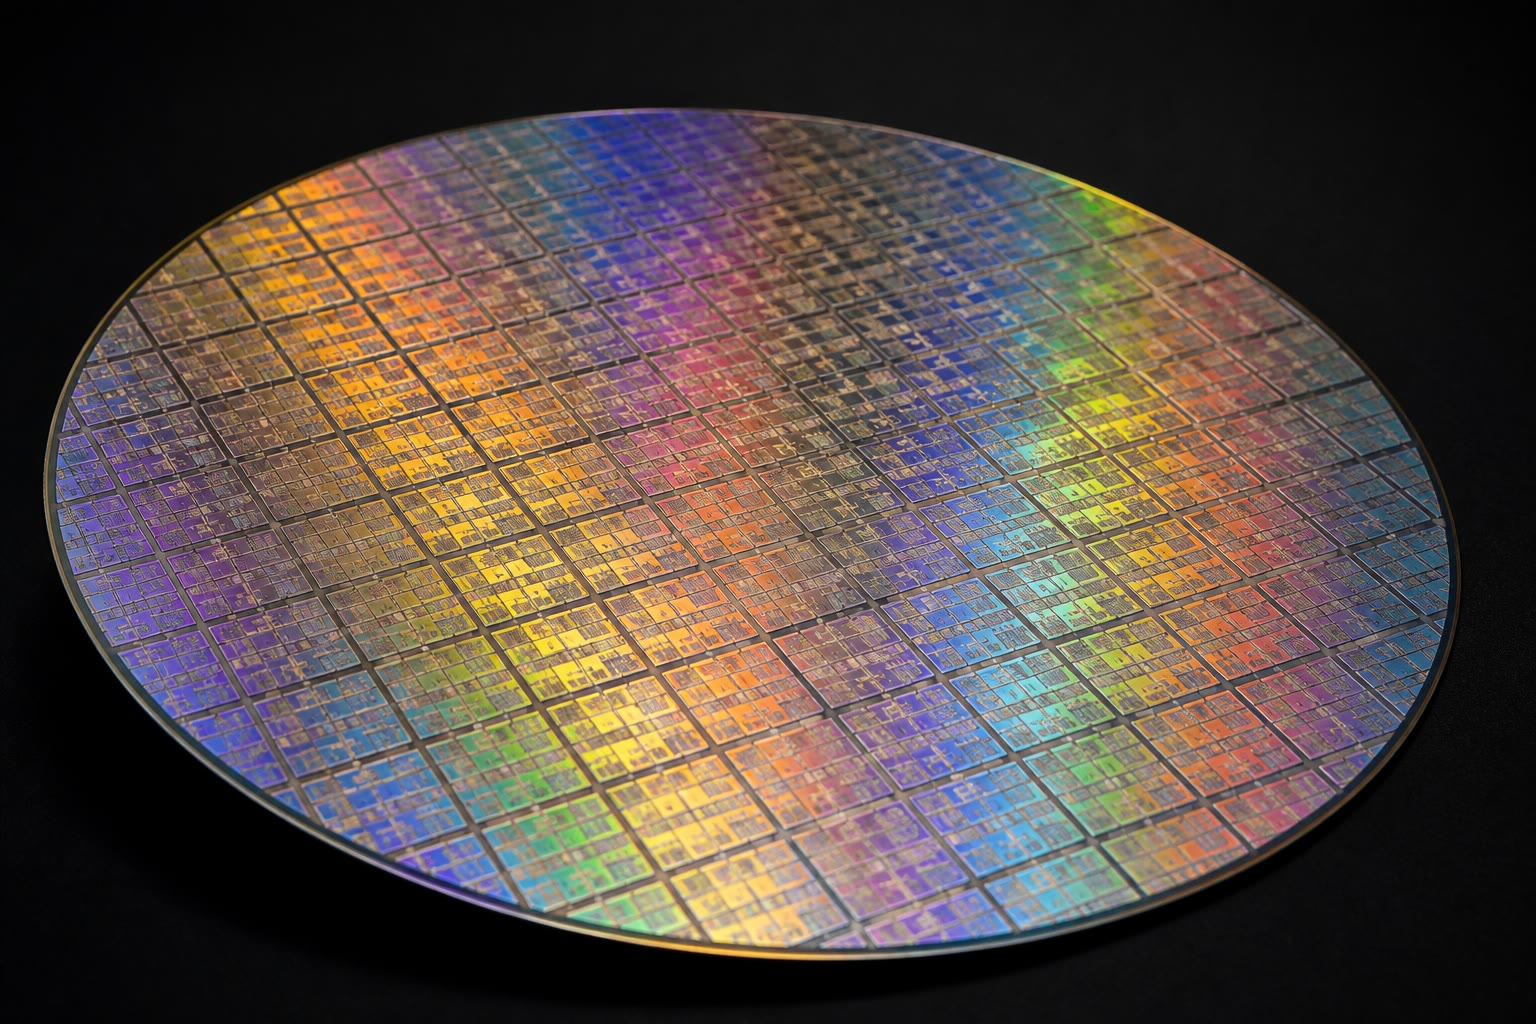
\includegraphics[width=0.58\linewidth]{images/book5/ai/b5-20-silicon-wafer.jpg}

{\small 一片成品硅晶圆：数百枚芯片，每枚含数十亿个结，全部印制于同一块\omterm{def:b3:electrons-in-solids:doping}{掺杂}\omterm{def:b3:crystalline-solids:lattice}{晶体}之上——能带理论，是二十世纪影响最深远的制造配方。}
\end{omfigure}

\section{练习}

\begin{exercise}[$\star$]\label{exo:b3:electrons-in-solids:1}
德鲁德的铜。$n = \qty{8.5e28}{m^{-3}}$，电阻率
$\rho = \qty{1.7e-8}{\ohm.m}$。计算 (a) $\tau =
m_{\text{e}}/ne^2\rho$；(b) 利用费米
速度 $v_{\text{F}} = \qty{1.6e6}{m/s}$ 求平均自由程；(c) 以
\omterm{def:b3:crystalline-solids:lattice}{晶格常数}（$a = \qty{3.61}{\angstrom}$）表示该自由程；(d) 解释为何
如此长的飞行已暗示，离子本身并不参与
散射。
\end{exercise}

\begin{exercise}[$\star$]\label{exo:b3:electrons-in-solids:2}
导线中的蜗牛。一根 \qty{1}{mm^2} 的铜导线通过
\qty{10}{A} 的电流。(a) 求\omterm{prop:b3:electrons-in-solids:drude}{漂移速度}。(b) 电子穿过一根
\qty{1}{m} 长的台灯电线需要多长时间？(c) 为何
灯仍会立即亮起？(d) 比较
$v_{\text{d}}$ 与 $v_{\text{F}}$，并评论德鲁德的
弹子球图像。
\end{exercise}

\begin{exercise}[$\star$]\label{exo:b3:electrons-in-solids:3}
按能带分类。依据能带填充规则，对下列材料分类：(a)
钠（一个价电子）；(b) 镁（两个价电子——却是
\omterm{def:b3:electrons-in-solids:classes}{金属}：其能带必须如何？）；(c) 金刚石
（$E_{\text{g}} = \qty{5.5}{eV}$）；(d) 硅
（$\qty{1.12}{eV}$）——并分别说明
$\dd\rho/\dd T$ 的符号。
\end{exercise}

\begin{exercise}[$\star$]\label{exo:b3:electrons-in-solids:4}
带隙与光子。(a) 与硅带隙相匹配的光子波长是多少，
以及硅在哪一光谱区域变得透明？
(b) 金刚石同理：为何它在
可见光区清澈？(c) 氮化镓发光二极管的 $E_{\text{g}} =
\qty{3.4}{eV}$：这设定了怎样的颜色边界，蓝色发光二极管为何
需要这种材料？(d) 为何红色发光二极管
在过驱动时熄灭为暗色，而不是微微发出白光？
\end{exercise}

\begin{exercise}[$\star\star$]\label{exo:b3:electrons-in-solids:5}
维德曼–弗兰兹定律。(a) 由铜的 $\kappa =
\qty{400}{W/(m.K)}$ 与 $\sigma = \qty{5.9e7}{S/m}$，在
\qty{300}{K} 下计算 $\kappa/\sigma T$。(b) 与
索末菲值 $L = \pi^2k_{\text{B}}^2/3e^2 =
\qty{2.44e-8}{W.\ohm/K^2}$ 比较。(c) 用一句话解释为何同一种
载流子将两种电导率联系在一起。(d) 炊具
及其手柄：用该定律解释厨房的材料
选择。
\end{exercise}

\begin{exercise}[$\star\star$]\label{exo:b3:electrons-in-solids:6}
热容的平反。(a) 德鲁德预测
$\tfrac32nk_{\text{B}}$ 来自电子：取铜的 $n$，
它会使晶格的
$3nk_{\text{B}}$（每个原子一个传导电子）增加多少比例？(b)
\Cref{ch:b3:quantum-statistics} 则给出 $C_{\text{el}}
\sim \tfrac{\pi^2}{2}nk_{\text{B}}(T/T_{\text{F}})$：计算
抑制因子 $T/T_{\text{F}}$ 在 \qty{300}{K} 时的值
（$T_{\text{F}} = \qty{8.1e4}{K}$）。(c) 为何电子项
反而在液氦温度下\emph{占优}
（回想晶格的 $T^3$）？(d) 哪一种测量，以
$C/T$ 对 $T^2$ 作图，能将两者分离？
\end{exercise}

\begin{exercise}[$\star\star$]\label{exo:b3:electrons-in-solids:7}
费米面与布里渊区相交。(a) 对于铜，计算
费米波长 $\lambda_{\text{F}} = 2\pi/k_{\text{F}}$，取 
$k_{\text{F}} = (3\pi^2n)^{1/3}$。(b) 与 $2a$ 比较：
费米面距布拉格条件有多近？(c) 从物理上解释
为何在 $k = \pi/a$ 处的两个驻波（电荷位于
离子上与位于离子之间）的能量必定不同。(d) 哪一个
\cref{exo:b3:electrons-in-solids:1} 中的实验事实，能由布洛赫无散射定理
最终解释？
\end{exercise}

\begin{exercise}[$\star\star$]\label{exo:b3:electrons-in-solids:8}
指数型温度计。本征硅中 $n_{\text{i}}
\propto \eu^{-E_{\text{g}}/2k_{\text{B}}T}$。(a) 计算 
\qty{400}{K} 与 \qty{300}{K} 下载流子密度之比。(b)
由此画出热敏电阻的电阻随温度变化的示意图，并
与铂丝的电阻相比较。(c) 为何指数中含因子 2
（何者是\emph{成对}产生的）？(d) 估算
使硅电子器件失效的温度，其原因是本征
载流子淹没了\omterm{def:b3:electrons-in-solids:doping}{掺杂}浓度 \qty{5e21}{m^{-3}}
($n_{\text{i}}(300\,\text{K}) \approx \qty{1e16}{m^{-3}}$).
\end{exercise}

\begin{exercise}[$\star\star$]\label{exo:b3:electrons-in-solids:9}
\omterm{def:b3:electrons-in-solids:doping}{掺杂}运算。硅的原子数密度为 $\qty{5e28}{\text{原子}/m^3}$。(a) 每
百万个硅原子中掺入一个磷原子：载流子密度为多少，
以及它与 $n_{\text{i}} \approx \qty{1e16}{m^{-3}}$ 之比为多少？(b)
百万分之一的杂质使电导率改变了多少倍？(c)
试说明\omterm{def:b3:electrons-in-solids:classes}{半导体}制造为何先将材料提纯至
\emph{十亿}分之几的杂质水平，然后才有意\omterm{def:b3:electrons-in-solids:doping}{掺杂}。(d) 估算
\omterm{def:b3:electrons-in-solids:doping}{施主}之间的平均距离，并与 
\cref{exo:b3:electrons-in-solids:10} 中的 \qty{2.4}{nm} 轨道相比较。
\end{exercise}

\begin{exercise}[$\star\star\star$]\label{exo:b3:electrons-in-solids:10}
\omterm{def:b3:electrons-in-solids:doping}{施主}视为氢原子。第五个磷电子
绕其 $+e$ 离子运动，该离子\emph{位于硅内部}：以 
$\varepsilon_{\text{r}} = 11.7$
（见\cref{ch:b3:electromagnetism-in-matter}），并将电子
的质量取为其有效能带质量 $m^* = 0.26\,m_{\text{e}}$。
(a) 对\cref{ch:b3:hydrogen-atom}中的氢原子结果进行标度变换：
证明 $E = \qty{13.6}{eV}\times(m^*/m_{\text{e}})/
\varepsilon_{\text{r}}^2$，并计算其值。(b) 与 
$k_{\text{B}}T$（\qty{300}{K}）相比较：\omterm{def:b3:electrons-in-solids:doping}{施主}是否电离？(c) 对
\omterm{thm:b3:hydrogen-atom:levels}{玻尔半径}作同样处理。(d) 该轨道跨越数十个
\omterm{def:b3:crystalline-solids:lattice}{晶胞}，试说明这一事实为何自洽地论证使用
$\varepsilon_{\text{r}}$ 与 $m^*$ 是合理的。
\end{exercise}

\begin{exercise}[$\star\star\star$]\label{exo:b3:electrons-in-solids:11}
PN 结的数值。一个硅二极管的 $N_{\text{a}} =
N_{\text{d}} = \qty{1e22}{m^{-3}}$, $n_{\text{i}} =
\qty{1e16}{m^{-3}}$，$T = \qty{300}{K}$。(a) 计算 
$V_{\text{bi}} = (k_{\text{B}}T/e)\ln(N_{\text{a}}N_{\text{d}}/
n_{\text{i}}^2)$。(b) 由二极管定律计算 
$+\qty{0.5}{V}$ 与 $-\qty{0.5}{V}$ 处电流之比。(c) 为何 
$I_0$ --- 因而反向漏电流 --- 大约每
升高 \qty{10}{K} 翻一番？(d) 由四个同类二极管组成的桥可将交流电变为直流电：
用文字简述该电路的思路。
\end{exercise}

\begin{exercise}[$\star\star\star$]\label{exo:b3:electrons-in-solids:12}
太阳能带隙设计。(a) 能量低于 $E_{\text{g}}$ 的光子
透过；能量高于 $E_{\text{g}}$ 的部分以热的形式
在皮秒量级内耗散。试说明选取 
$E_{\text{g}}$ 时的权衡。(b) \qty{1.3}{eV} 附近的最优值
使单结效率上限约为三分之一
（肖克利–奎伊瑟）：硅
（\qty{1.12}{eV}）位于何处？(c) 为何叠层电池（宽带隙
电池位于窄带隙电池之上）能突破该上限？(d) 为何 
\emph{热}的太阳能电池板性能更差？（两个符合本章的理由：
二极管定律中的 $I_0$，以及带隙随 $T$ 的微小收缩。）
\end{exercise}

\begin{omfigure}
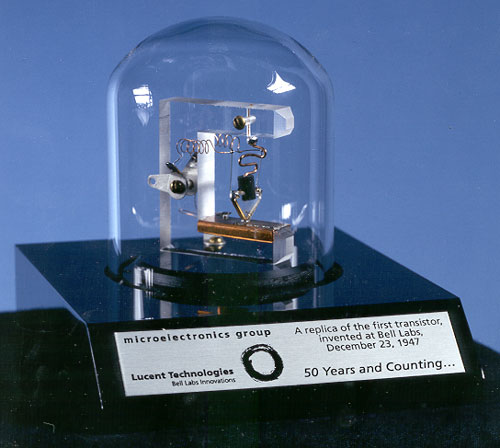
\includegraphics[width=0.45\linewidth]{images/book5/photo-first-transistor.jpg}

{\small 第一只\omterm{def:b3:crystalline-solids:lattice}{晶体}管的复制品（贝尔实验室，1947 年，公有领域）：两个金触点压在一小片锗上。能带理论的第一台机器 --- 经由传承，其余一切器件皆由此而来。}
\end{omfigure}

\section{问题：屋顶公投}

\begin{problem}\label{pb:b3:electrons-in-solids:1}
\emph{屋顶公投。}您的邻居正在决定是否
用光伏板为房屋做屋顶，并聘请您这位物理学家
担任仲裁人。候选面板为硅材料，
面积 \qty{2}{m^2}，六十块电池串联，额定功率为 \qty{400}{W}，
标准条件为正午阳光辐照度 \qty{1000}{W/m^2}。

\medskip\noindent\textbf{第一部分 --- 阳光与带隙相遇。}

\begin{enumerate}
  \item 太阳光近似为 \qty{5800}{K} 的热辐射谱
        （见\cref{ch:b3:photons-phonons}）：计算其
        峰值光子（维恩）的能量，以 eV 为单位。
  \item 硅的带隙为 \qty{1.12}{eV}：硅电池能够
        收集的最长波长是多少？
  \item 约五分之一的太阳功率以
        能量低于带隙的光子形式到达。这部分能量在电池板中会如何？
  \item 一个 \qty{2.5}{eV} 的绿色光子被吸收：其能量中有多少
        以电子–\omterm{def:b3:electrons-in-solids:doping}{空穴}对能量的形式保留，其余去向何处，
        以及这一过程发生得多快？
  \item 综合第 3 与第 4 小题，得到光谱的结论：入射功率约
        一半在任何电子学过程开始之前就已损失。
        请分别用一句话陈述两种损失途径。
  \item 光子为何根本需要 $\ge E_{\text{g}}$ --- 是什么
        阻止普通硅在短时间内
        相继吸收两个半带隙光子？
\end{enumerate}

\medskip\noindent\textbf{第二部分 --- 作为引擎的结。}

\begin{enumerate}[resume]
  \item 每个电池单元都是一个 p--n 结。用三句话说明\omterm{prop:b3:electrons-in-solids:junction}{耗尽区}的内建电场
        如何把产生的电子–\omterm{def:b3:electrons-in-solids:doping}{空穴}对变为外电流——
        哪种载流子沿哪个方向运动，
        以及它们为何不会简单地复合。
  \item 已知 $N_{\text{a}} = N_{\text{d}} = \qty{1e22}{m^{-3}}$
        且 $n_{\text{i}} = \qty{1e16}{m^{-3}}$，
        求 \qty{300}{K} 时的 $V_{\text{bi}}$。
  \item 一个正常工作的电池单元约输出 \qty{0.6}{V}。
        六十个单元串联，则电池板的工作电压是多少？
  \item 由 \qty{400}{W} 的额定功率推出
        工作电流。
  \item 估算电池板有效吸收的光子通量（每秒光子数），取
        每个被吸收光子 $\sim\qty{2}{eV}$，
        并与电流所对应的电子通量比较：被吸收光子中
        有多大比例产生了
        被收集的电子？
  \item 额定效率：由入射的 \qty{2000}{W} 得到 \qty{400}{W}。
        请将 20\,\% 与第一部分中“电子器件之前已有一半损失”相调和：
        其余的三十个百分点
        去了哪里？
  \item 为何电池单元输出 \qty{0.6}{V}，而非带隙对应的完整
        \qty{1.12}{V}？
        （请在二极管定律中指出元凶。）
\end{enumerate}

\medskip\noindent\textbf{第三部分 --- 真实的屋顶。}

\begin{enumerate}[resume]
  \item 北纬 $50^\circ$ 处一个无云的冬季正午，
        光以 $30^\circ$ 仰角照射。
        求水平放置的电池板相对于法向入射的
        几何因子。
  \item 电池板数据手册给出输出的 $-0.4\,\%/\text{K}$：
        夏季时，黑色屋顶上的电池板温度可达 \qty{65}{\celsius}。
        额定功率中还能保留多少？
  \item 结合
        \cref{exo:b3:electrons-in-solids:12}(d) 解释温度造成的损失。
  \item 一个烟囱遮住了六十个单元中的一个。为何这一个单元
        就足以扼制整个串联链路 --- 而该单元自身的二极管特性
        又会对这个被遮挡的单元产生什么影响？
  \item 制造商在每个子串两端并联一个\emph{旁路二极管}，
        请用一句话说明它的作用。
  \item 按日和天气平均计算，屋顶实际输出
        为额定功率的 \qty{15}{\percent}。估算这块 \qty{400}{W} 电池板一年的能量，
        以千瓦时为单位。
\end{enumerate}

\medskip\noindent\textbf{第四部分 --- 结论。}

\begin{enumerate}[resume]
  \item 每千瓦时按 \qty{0.25}{euros} 计，这块电池板一年能赚多少？
        若安装成本为 \qty{300}{euros}，
        回收期是多久？
  \item 制造这块电池板大约耗费 \qty{500}{kWh} 能量
        （硅须通过熔化来提纯），
        需要多长时间才能收回自身的能量？
  \item 你的邻居问：为什么不能干脆把电池板“涂黑”，
        以捕获低于带隙的那五分之一？请用能带理论
        用两句话作答。
  \item 他们接着问：为何不在下方再叠一块带隙更小的
        电池板？请结合
        \cref{exo:b3:electrons-in-solids:12}(c) 作答，
        并指出其实际困难。
  \item 三十年后，电池板的输出衰减至额定值的 85\,\%。
        本章中哪些微观元凶可能使
        （回想一下限制 $\tau$ 的是什么，以及结惧怕什么）
        最有可能使电池单元老化？
  \item 以四句话给出仲裁者的总结：带隙物理决定能量收获；
        结将其转化为电能；串联接线与温度使其打折；
        而能量与欧元的账目 --- 
        最终对电池板有利。
\end{enumerate}
\end{problem}
